\section{世界與相機}
\label{sec:world}

\subsection{地形與 Chunk}

作業要求的地板是 $[0,0,0]$ 到 $[50,0,50]$ 的平面，本作業改為依 seed 生成的起伏地形，並以邊長 16 m 的 chunk 為單位，只載入機器人周圍半徑 12 個 chunk 內的範圍；機器人移動時，遠處的 chunk 會被釋放、前方的 chunk 被生成，地面因此沒有邊界（圖~\ref{fig:terrain}）。

地形高度由自己實作的 Perlin 雜訊疊加而成：以多層頻率加倍、振幅減半的雜訊（fBm）組成大陸性、崎嶇度、溫度與濕度等場，再依崎嶇度決定哪裡長出丘陵、山脈或海岸斷崖。
每一格再依高度、坡度、溫度與濕度分類成平原、沙漠、雪原、海洋等生態系，決定地表的顏色，並畫成棋盤格，讓平坦的地面也看得出距離與移動。
每個 chunk 的隨機數由世界 seed 與 chunk 座標雜湊而來，同一個 seed 不論以什麼順序載入，生成的世界都相同。

每個 chunk 的地形網格在第一次繪製時建立並快取，之後每幀只需重畫網格，不必重新取樣雜訊；改成快取後幀率從約 40 FPS 回到 60 FPS。
出生點從原點往外以螺旋狀搜尋，選擇第一個高度至少 1 m 的陸地，避免一開始就掉進水裡。

\subsection{障礙物}

每個 chunk 在固定的三個位置分別放置一個方塊、一個球與一個圓柱，位置落在水面或冰面上時略過。
方塊的長寬高與旋轉角度、球的半徑、圓柱的半徑與高度都由該位置的 seed 隨機決定，大小上限為 2 m，顏色也依 seed 隨機產生。
障礙物底部貼齊所在位置的地面高度，與地形一樣以網格繪製，並套用第~\ref{sec:robot} 節的 Half-Lambert 明暗計算。

\begin{figure}[htbp]
    \centering
    \begin{subfigure}[t]{.48\textwidth}
        \centering
        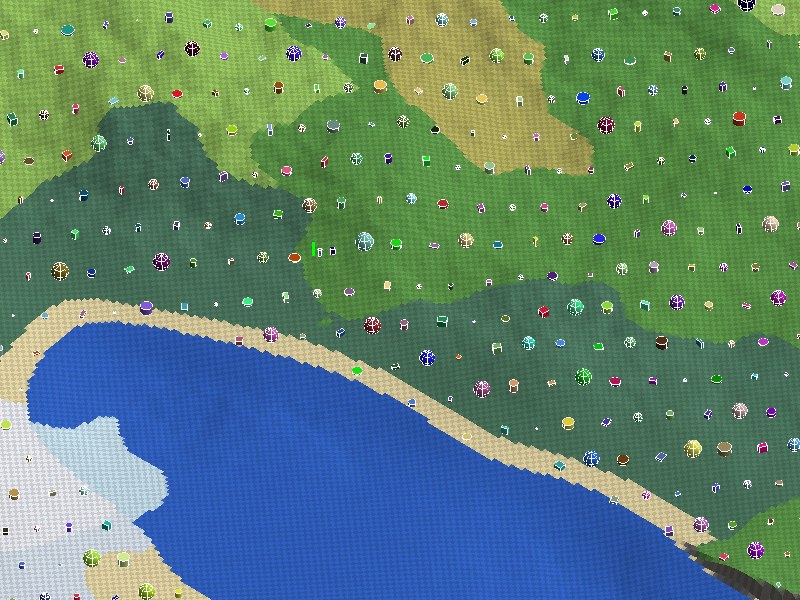
\includegraphics[width=\linewidth]{docs/figures/terrain-overview.png}
        \caption{拉遠後的地形與生態系}
    \end{subfigure}\hfill
    \begin{subfigure}[t]{.48\textwidth}
        \centering
        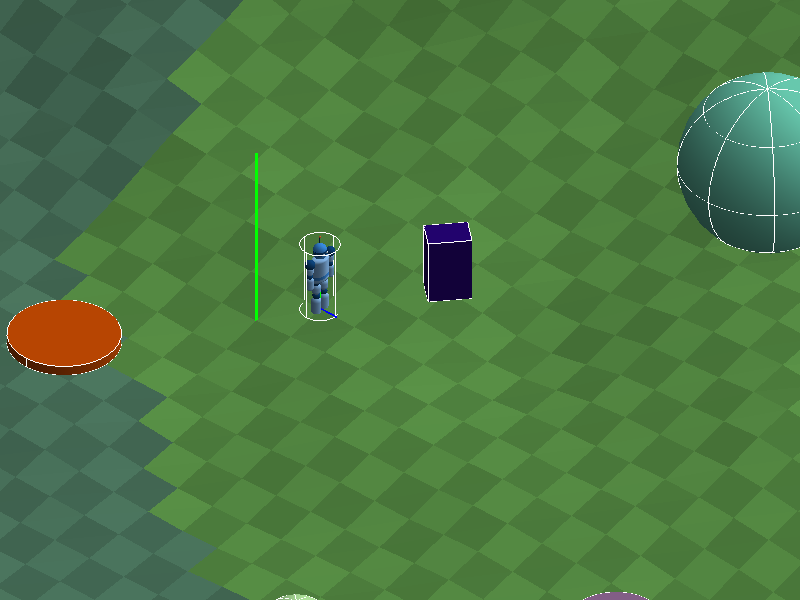
\includegraphics[width=\linewidth]{docs/figures/obstacles.png}
        \caption{方塊、球與圓柱障礙物}
    \end{subfigure}
    \caption{地形與障礙物}
    \label{fig:terrain}
\end{figure}

\subsection{相機與投影}

相機以 eye、focus、up 三個參數描述，對應 \lstinline|gluLookAt|；投影沿用作業給定的 \lstinline|glOrtho| 平行投影。
focus 是機器人眼睛的位置（第~\ref{sec:scene-graph} 節的正向運動學），eye 則依相機的 yaw、pitch 從 focus 往後退一段距離：
\begin{equation*}
    \mathbf{f} = (-\sin\psi\cos\theta,\; \sin\theta,\; -\cos\psi\cos\theta), \qquad \text{eye} = \text{focus} - d\,\mathbf{f},
\end{equation*}
其中 $\psi$、$\theta$ 為相機的 yaw 與 pitch，$\mathbf{f}$ 是 $(0, 0, -1)$ 先俯仰再繞 $y$ 軸旋轉後的視線方向；pitch 限制在 $\pm 89.9^\circ$ 內，避免視線與 up 向量平行。

平行投影的畫面大小與距離無關，因此「拉近」是縮小 \lstinline|glOrtho| 的左右上下範圍：基本範圍為 $\pm 48 \times \pm 40$，除以 0.5 到 24 倍的縮放倍率。
範圍會依視窗的長寬比調整，視窗改變大小時畫面不會變形。
平行投影中 eye 只決定裁切範圍，near 取 $-400$、far 取 $400$，眼睛背後的高地與遠處整個載入範圍的地形才不會被切掉。
每幀先畫 3D 場景，再切換成以像素為單位的 \lstinline|glOrtho| 畫出 HUD。
